% set the document type and the font size
\documentclass[12pt]{article}

% use Spanish package
\usepackage[spanish]{babel}

% set UTF-8 codification
\usepackage[utf8]{inputenc}

% insert images
\usepackage{graphicx}
\graphicspath{ {images/} }

% insert graphical tree
\usepackage{tikz}
\usepackage{tikz-qtree}

% no equation numeration
\usepackage{amsmath}

% set contents to page using [H]
\usepackage{float}

% create the title
\title{\textbf{Sistemas Digitales}}
\date{2017-09-26}
\author{Diego Enrique Fontán, CosasDePuma}

\begin{document}
	% no page numbers
	\pagenumbering{gobble}

	% title
	\maketitle
	\newpage
	
	% table of contents
	\tableofcontents
	\newpage
	
	% arabic numeration
	\pagenumbering{arabic}
	
	\section{Introducción a los Sistemas Digitales}
	
		\vfill
	
		\subsection{Tipos de señales}
			
			Tipos de señales que nos podemos encontrar en relación a los valores que pueden tomar:\\
		
			- \textbf{Señales analógicas:} Pueden tomar infinitos valores distintos a lo largo del tiempo.\\
		
			- \textbf{Señales digitales:} Sólo pueden tomar un número finito de valores distintos a lo largo del tiempo.\\
				
			\begin{figure}[H]
			\centering
			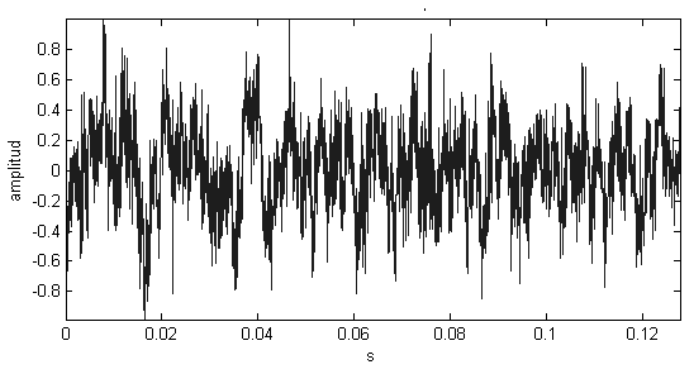
\includegraphics[width=150px,height=100px]{analogic}
			\caption{Ejemplo de señal analógica}
			\end{figure}
		
			\begin{figure}[H]
			\centering
			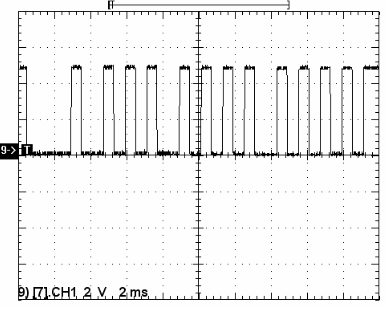
\includegraphics[width=140px,height=100px]{digital}
			\caption{Ejemplo de señal digital}
			\end{figure}
			
			\newpage
	
		\subsection{Señales binarias}
	
			Las señales binarias son un caso particular de las señales digitales.\\
			
			Se caracterizan porque sólo pueden tomar dos valores distintos a lo largo del tiempo.\\
	
			Los sistemas electrónicos digitales que se utilizan hoy en día operan con señales binarias.\\
			
			Por lo tanto, según el valor que tome la señal en cada momento, se pueden determinar dos estados diferentes que posteriormente se emparejarán a números binarios.\\
			
			\begin{figure}[H]
			\centering
			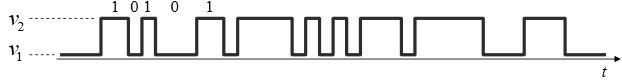
\includegraphics[width=250px,height=50px]{binary}
			\caption{Ejemplo de señal binaria}
			\end{figure}
			
			El que se denomine a los sistemas que utilizan estas señales como \textit{sistemas digitales} en vez de \textit{sitemas binarios} se debe a que, en general, procesan valores digitales, los cuales se codifican mediante combinaciones de valores binarios para que puedan ser tratados.\\
			
		\subsection{Ventajas de los sistemas digitales}
		
			Las ventajas que tienen los sistemas digitales respecto a los analógicos son, entre otras:\\
			
			- Son más fáciles de diseñar.
			
			- Son menos sensibles a agentes externos (como a las interferencias).
			
			- Permiten almacenar y operar con grandes cantidades de información de forma rápida y segura.
			
			
			
			\newpage
			
	\section{Sistemas de numeración y códigos binarios}
	
		\vfill
		
		Un sistema de numeración no es más que un método que se usa para representar cantidades de forma simbólica, siguiendo ciertas normas y convenios.\\
		
		Un número es una representación mediante símbolos de una cantidad dada.\\
		
		Una misma cantidad puede ser representada mediante un número distinto en función del sistema de numeración que se considere.\\
		
		Por ejemplo:\\
		
		\[
		12_{10} = C_{16} = 14_{8} = 1100_{2}
		\]
	
		Los sistemas de numeración sólamente expresan el módulo, magnitud o valor absoluto de una cantidad, nunca si es positiva o negativa.\\
		
		Hoy en día utilizamos sistemas de numeración posicionales, caracterizados por:\\
		
		- Las cantidades se representan mediante una sucesión ordenada de números a ambos lados de un símbolo de referencia (punto, coma...)\\
		
		\begin{figure}[H]
			\centering
			\Tree [.Cantidad  [.3735928559 real ] [., símbolo ] [.129152485 fraccionaria ] ]
		\end{figure}
		
		- Cada dígito tiene asociado un \textbf{peso} cuyo valor depende de la \textbf{base} y de la \textbf{posición} que ocupe el dígito.\\
		
		\newpage
		
		\subsection{Peso numérico según la base y posición}
		
			Las posiciones y los pesos asociados a cada uno de los dígitos de una cantidad guardan la siguiente relación:
			
			\begin{equation}
			\notag
			\overbrace{\underbrace{{a}_{n-1}^{{b}^{n-1}}\ {a}_{n-2}^{{b}^{n-2}}\ ...\ {a}_{1}^{b}\ {a}_{0}^{1}}_{parte\ real}\ ,\ \underbrace{{a}_{-1}^{{b}^{-1}}\ {a}_{-2}^{{b}^{-2}}\ ...\ {a}_{-(m-1)}^{{b}^{-(m-1)}}\ {a}_{-m}^{{b}^{-m}}}_{parte\ fraccionaria}}^{pesos}
			\end{equation}
        
	
\end{document}
